\documentclass[../main.tex]{subfiles}
\begin{document}
\setchapterimage[6.5cm]{Images/final.jpg}
\setchapterpreamble[u]{\margintoc}
\chapter[Final Topics]{Final Topics\footnotemark[0]}
\labch{extra}
These are the final topics of the course, objects of January lectures. The lectures about the hierarchy problem have been done by prof. Contino while prof. Nardecchia did the lectures about the CP violation. I did not know where to put these topics inside the various chapters so I decided to give them a special extra chapter.
\section{Hierarchy Problem of the Standard Model}
\subsection{Naturalness of a Theory}
To start our discussion, we first have to define what is a \textbf{natural theory}. If we take a list of observables and the theory describes their values in a natural way without requiring any cancellation, then the theory is called natural. A sublist of observables is used as input observables and since we need predictability the number of observables has to be larger than the number of input observables. We are usually interested in certain kinds of observables, e.g. masses, and we want to say whether the value of a certain observable is naturally reproduced by the theory then this observable should not be one of the input observables. If it is one of the input observables it is not possible to determine whether its value is naturally reproduced or not. For example, in QED the mass of the electron and the value of the coupling are input parameters, so it does not make much sense to ask ourselves if these values are natural or not. If we have a third observable and make a prediction, then at this point we can ask if they are naturally reproduced in the theory or not. We have predictions for these observables, so for each one we have relations of this kind:
\[
f_j(\{O_i\})=0 \quad j=1,\cdots,\text{\# predicted observables}
\]
There is one relation for every predicted observable, the function depends on all possible observables. These are relation among physical quantities, they have nothing to do on the dependence on the renormalization scheme. These predictions are naturally reproducing the experimental values if there is no cancellation among the different terms in the function $f_j$.\\
Suppose to have only one observable as prediction while the others are input and we want to know if the theory predicts naturally the value of this observable. If, in order to obtain the value of this predicted observable, we have to choose very carefully the values of the input ones because otherwise the relation does not give us the desired value, then it means that the theory is not naturally reproducing this observable. This is the unnatural situation.\\
Here everything is formulated in terms of observables although it is not what it is found in literature. This is because the perturbative series in QFT is never convergent, which means that eventually we have to truncate it and after truncation we will never get relations which are free from uncertainties and dependence on the renormalization scheme. They are never exactly physical quantities, they always have some degree of theoretical dependence. The second observation is that the theory will have a lot of theoretical parameters, so if we want to make several predictions and we want to vary the input observables consistently with the theory, that might be a bit cumbersome. We can instead vary directly the parameters in the Lagrangian in such a way that the input observables vary in the region we are interested in.\\
The absence of tuning can be expressed by a criterion. Let's say that $a_i$ are the Lagrangian parameters and we want to taste whether the value of a certain observables $O_j$ is naturally reproduced or not. 
\[
\left|\frac{a_i}{O_j}\frac{\partial}{\partial a_i}O_j(\{a_i\})\right|<\Delta \quad \forall i,j
\]
This is the \textbf{Barbieri-Giudice criterion}. The naturalness is expressed in terms of variation of the observables with respect to the Lagrangian parameter but only because by varying the parameters we are varying the input observables. What we are interested in is whether this predicted observable is natural after varying the input observables, i.e. the parameters of the Lagrangian. An unnatural situation is the one in which in order to reproduce the value of $O$ we need to choose very carefully these $a_i$.\\
There is another work which appeared before the one by Barbieri and Giudice and it was made by t'Hooft, who proposed another criterion to decide whether a theory was natural or not. He wanted to see if small values of a certain observable were natural or not and it is better to rephrase all the dimensionful parameters in terms of dimensionless ones. At this point, t'Hooft asked himself if the measured value for a certain quantity was natural or not. He proposed the rule which states that \textit{it is natural if, by sending to zero the value of that dimensionless parameter, the theory acquires a larger symmetry.}
\subsection{Naturalness of the Electroweak Scale}
We now want to apply this naturalness criterion to the electroweak scale since the hierarchy problem is a problem of naturalness of the EW scale in the Standard Model.\\
First of all, we make an example and take the QCD scale, which can be predicted within the QCD theory. It is a prediction in the sense that we can measure the value of the coupling at a certain scale $g_S(M)$, e.g. a very high-energy scale where QCD is perturbative, by measuring a scattering process. This is our input and it is dimensionless. At this point, we note that moving to lower energy the coupling becomes stronger and stronger until it gets non perturbative $g_S(\Lambda)\approx4\pi$, where this $\Lambda$ as usual is given by:
\[
\Lambda_{\text{QCD}}=M\exp{-\frac{8\pi^2}{\beta_0}\frac{1}{g_S(M)}}
\]
This is just an estimate for the QCD physical scale obtained at one-loop. From this, we can understand why $\Lambda_{\text{QCD}}\ll M$ is natural. Because here there is an exponential dependence on the value of the coupling, so if the coupling is small the exponential becomes very small and $\Lambda_{\text{QCD}}$ is exponentially suppressed with respect to $M$. There is no cancellation we require to get the situation of this kind, the theory in which $\Lambda_{\text{QCD}}$ is much smaller than another UV scale is naturally reproduced. In order to do this, it is crucial that the QCD scale is predictable otherwise if it had to be an input parameter then we could not ask whether this scale is natural or not. There is this mechanism which transforms a dimensionless quantity into a dimensionful one and it goes under the name of \textbf{dimensional transmutation}.\\
Now we can require the same thing for the EW scale which is different from the previous example. First of all it is not predictable because the EW scale is set by the Higgs mass term, which can be defined in terms of the vev $v^2=\mu^2/\lambda$ and $\mu^2$ is the coefficient for the Higgs mass term, $-\mu^2H^\dagger H$. It is directly a parameter of the Lagrangian, so the scale we want to test is not calculable, it is an input parameter. The EW scale is not predictable within the SM so it does not make sense to ask whether it is natural or not. However, the SM is not a full theory, is an EFT. If we think of the SM as embedded in a larger UV completion there is a possibility that the mass term of the Higgs can be computed in the full theory. If it is not calculable then there is no problem, there is no naturalness, it is just an input parameter of the Lagrangian and end of the story. The question of whether it is natural or not stands only if the mass term of the EW scale is calculable in the full theory and at this point it makes sense to ask if it is natural or not.\\
The question about its naturalness makes no sense at all in the SM since it is an input quantity, it has sense only if we think of the SM as part of a larger theory in which the mass term of the Higgs is, hopefully, calculable. There then should be other particles in the full theory, which have not been discovered yet, that cancel the quadratic divergence arising at loop level from the exchange of SM particles. We know the mass term of the Higgs is quadratically divergent within the SM, these are the one-loop corrections to it:\marginnote{Notice that we are not talking about the Higgs physical mass, only about the Higgs mass term.}
\begin{figure}[h]
    \centering
    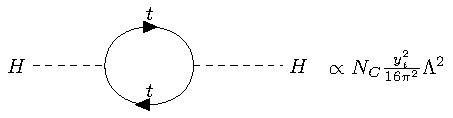
\includegraphics[width=0.8\textwidth]{Images/hc1.pdf}
    \caption*{}
    \labfig{hc1}
\end{figure}\\
Since the contribution coming from loop of fermions is proportional to the square of the Yukawa coupling, we consider the contribution coming form the top. To be more precise, the contribution of this diagram is:
\[
\delta\mu^2=N_C\frac{y_t^2}{8\pi^2}\Lambda^2 \qquad y_t^2=\frac{2m_t^2}{v^2}
\]
where $v=246$\,GeV and $m_t=173$\,GeV. This formula is interpreting $\Lambda$ as a hard cut-off in the loop. There is also the correction coming from the gauge fields:
\begin{figure}[h]
    \centering
    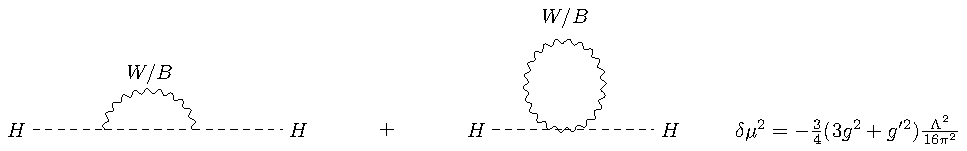
\includegraphics[width=\textwidth]{Images/hc2.pdf}
    \caption*{}
    \labfig{hc2}
\end{figure}\\
which gives us a contribution equal to:
\[
\delta\mu^2=-\frac{3}{4}(3g^2+g'^2)\frac{\Lambda^2}{16\pi^2}
\]
Here the sign of the correction is negative. That is because first of all we are defining $\mu^2$ to be positive in presence of EW symmetry breaking. Moreover, there is a contribution from Higgs self interaction:
\begin{figure}[h]
    \centering
    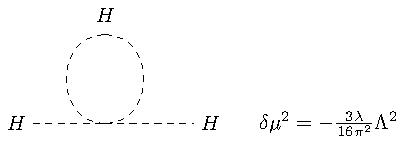
\includegraphics[width=0.7\textwidth]{Images/hc3.pdf}
    \caption*{}
    \labfig{hc3}
\end{figure}\\
We are looking at these divergencies because we have a counter term in the theory, $H^\dagger H$, to reabsorb the divergencies. If the full theory is such that the EW scale is calculable it means there is no counter term: where there is a counter term there is a divergence and then $\mu^2$ is an input. In the full theory, the Higgs mass term should not be divergent, there should be some symmetry which forbids writing such term or at least forbids the occurrence of divergencies. Hence, if we relax the theory there would be necessary other particles which remove these divergencies. This is the SM contribution, if we add new particles then the sum has to be finite and the divergence will be canceled. The partners of the top will give a new contribution, each of these contribution will go like $\Lambda^2$ and in order for the sum to be finite they need to have opposite signs. If we integrate out these heavy partners at the scale $M$ and then do matching with an EFT which is the SM just below the scale $M$, we have a divergence. The divergence is removed exactly at the scale $M$, which will appear in the finite contribution and that is what we want to estimate.\\
We have three sets of contribution, from the top, the gauge fields and self interaction, each of them going like some scale of heavy particles which remove the divergence. These three contribution, in the case $M$ is much larger than the EW scale, which is the hypothesis we want to test, are of order of this scale then there is a problem because they will be much much larger than the EW scale. 
\[
\left\{
\begin{aligned}
&\delta\mu^2(\text{top})+\delta\mu^2(\text{gauge})+\delta\mu^2(\text{Higgs})\simeq\lambda v^2\ll M^2\\
&\delta m_h^2(\text{top})+\delta m_h^2(\text{gauge})+\delta m_h^2(\text{Higgs})=(125\,\text{GeV})^2
\end{aligned}
\right.
\]
This is the \textbf{hierarchy problem}, the sum of these contribution will have to cancel very precisely because each of them is of order $M^2$ times a loop factor which at best can be $10^{-3}$ in such a way that we get something of the order of the EW scale. It does not seem natural to get an EW scale which is much much smaller than some much heavier physical scale.\\
For example, if we take $M=10$\,TeV then we get:
\[
\delta m_h^2(\text{top})=(2.7\,\text{TeV})^2 \quad \delta m_h^2(\text{gauge})=-(1.1\,\text{TeV})^2 \quad \delta m_h^2(\text{Higgs})=-(1.0\,\text{TeV})^2
\]
These numbers are much larger than 125 GeV individually. In the full theory they have some coefficients in front that we cannot predict unless the full model is known, the divergencies are not calculable precisely, just estimates. There has to be some cancellation among these three contributions in such a way that their sum is (125\,GeV)$^2$ to reproduce the experimental value. This means that there will be a fine tuning which in general can be estimated to be approximately equal to:
\[
\frac{m_h^2\Bigr|_{\substack{\text{exp}}}}{\delta m_h^2(\text{top})}=\left(\frac{456\,\text{GeV}}{\Lambda}\right)^2
\]
Only the contribution from the top was considered being it the largest one. $\Lambda$ cannot be much bigger than 500\,GeV otherwise there will be a tuning, this tuning is a small number in the definition and if we set $\Lambda=10$\,TeV there will be something of the order of 0.2\%.\\
The moral is that if the full theory is one where the EW scale, hence the mass of the Higgs boson, is calculable in terms of other input quantities then there has to be new particles which remove the quadratic divergencies at the level of $(1-2)$\,TeV but not much higher. This was the motivation to build the LHC.
\subsection{Applications of Naturalness Arguments}
To see why we should trust this argument, we see two examples: the GIM mechanism and the electromagnetic corrections to the pion mass.\\
Let's start with the GIM mechanism. At the time, there was an SU$(2)\times$U(1) electroweak theory proposed by Glashow and then Weinberg and Salam lately. However, it was a theory for leptons because at the time only three quarks were known: up, down and strange. The EW interactions of these quarks were still described by the Fermi theory, with an interaction of the form:
\[
\pazocal{L}=-\frac{G_{\text{F}}}{\sqrt{2}}(J_\mu^{\text{had}}+J_\mu^{\text{lep}})(J_\mu^{\text{had}}+J_\mu^{\text{lep}}) \quad \text{where:}\;\left\{
\begin{aligned}
&J_\mu^{\text{lep}}&=\overline{e}\gamma^\mu(1-\gamma_5)\nu_e+\overline{\mu}\gamma^\mu(1-\gamma_5)\nu_\mu\\
&J_\mu^{\text{had}}&=\overline{u}\gamma^\mu(1-\gamma_5)(\cos\theta_cd+\sin\theta_cs)
\end{aligned}
\right.
\]
This was the four-fermion interaction and it worked fine. Problems came when people used this Lagrangian at one-loop, which lead to the prediction of the existence of flavour changing neutral current (FCNC). In particular, at the time people were very much concerned about process in which strangeness was changed by two unity, in particular the $K\overline{K}$ oscillations. Using this Lagrangian gives us two kind of diagrams:
\begin{figure}[h]
    \centering
    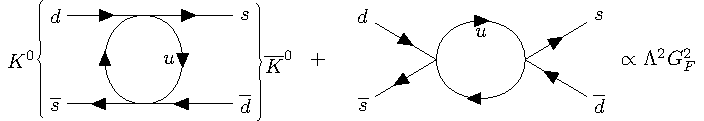
\includegraphics{Images/kk.pdf}
    \caption*{}
    \labfig{kk}
\end{figure}\\
These diagrams are quadratically divergent but people knew this was an EFT but the main problem regarded which value $\Lambda$ could have. It was already known that these interaction originated from the exchange of the $W$, so eventually the value of the cut-off is given by $m_W$, which was not known at the time. In order to predict it, it was necessary to know the value of the coupling, being $m_W^2=g^2v^2/4$. $G_{\text{F}}$ is given in term of $v^2$ but in order to know $g$ we need two measurements: the electromagnetic fine structure constant and the mixing angle $\theta_w$. 
\[
\frac{1}{e^2}=\frac{1}{g^2}+\frac{1}{g'^2} \qquad g\sin\theta_w=e
\]
The measurement of $\sin\theta_w$ came only in 1973 by the Gargamelle experiment at CERN. This came only later, at the time the value of $m_W$ was unknown but they knew that these relations held true.\\
The real part of the amplitude of the scattering in the above diagrams, denoted by $A_{12}$, is connected with $\Delta m_K=m_{K_L}-m_{K_S}=3.5\cdot10^{-12}$\,MeV and if we use this estimate $\Lambda$ turns out to be of order 3\,GeV. This is a problem: if we know that $m_W$ is connected to $G_{\text{F}}$ then it is possible to see that $m_W$ can be interpreted in terms of $\Lambda$, resulting in $g\sim10^{-4}$. If $g$ is much much smaller than $e$, then this relation does not work anymore. This chain of logical consequences lead to a puzzle and the way out was the proposal that the cut-off is not $m_W$ but it is the mass of something much lighter, the charm quark.\\
Glashow, Iliopoulos and Maiani then proceeded to extend the Fermi interaction to include the \nth{4} proposed quark, the hadronic current $J^\mu_{\text{had}}$ gets now modified as:
\[
J^\mu_{\text{had}}=\begin{pmatrix}
    \overline{c} & \overline{u}
\end{pmatrix}\underbrace{\begin{pmatrix}
    \cos\theta_c & \sin\theta_c\\
    -\sin\theta_c & \cos\theta_c
\end{pmatrix}}_{V}\gamma^\mu(1-\gamma_5)\begin{pmatrix}
    s\\d
\end{pmatrix}
\]
As it is possible to see, there is a part already known involving just $\overline{u}, d$ and $s$ and the extension which regards the charm quark. $V$ is a unitary, real, orthogonal matrix and it is now possible to reformulate the amplitude $\pazocal{A}$ of the $K\overline{K}$ oscillations in terms of elements of $V$:
\[
\pazocal{A}\propto G_{\text{F}}^2\sum_{i,j}V_{id}V_{is}^*V_{jd}V_{js}^*F(m_i,m_j)
\]
where $F$ is a loop function of dimension 2 such that $F(x,y)=F(y,x)$. It is common to define the following quantities:
\[
\lambda_u:=V_{ud}V_{us}^* \qquad \lambda_c:=V_{cd}V_{cs}^*
\]
The unitarity of $V$ implies that $\lambda_u+\lambda_c=0$:
\[
\lambda_u+\lambda_c=\sum_{i=u,c}V_{id}V_{is}^*=(V^\dagger V)_{sd}=0\Rightarow\lambda_u=-\lambda_c
\]
Using this, the amplitude $A(K\overline{K})$ gets written as:
\begin{align*}
\pazocal{A}&=G_{\text{F}}^2\left[\lambda_c^2F(m_c,m_c)+\lambda_u^2F(m_u,m_u)+2\lambda_c\lambda_uF(m_c,m_u)\right]\\
&=G_{\text{F}}^2\lambda_c^2\left[F(m_c,m_c)+F(m_u,m_u)-2F(m_c,m_u)\right]
\end{align*}
The loop function is quadratically divergent:
\[
F(m_i,m_j)\simeq\Lambda^2+m_im_j\log\Lambda f(m_i/m_j)+\text{finite terms}
\]
The amplitude however is not quadratically divergent, the divergence cancels out in virtue of the fact that:
\[
\lambda_u^2+\lambda_c^2+2\lambda_u\lambda_c=(\lambda_u+\lambda_c)^2=0
\]
Moreover, the log-divergence cancels out by accident therefore we are left only with the finite part. In the limit $m_u\ll m_c$, the amplitude becomes:
\[
\pazocal{A}=G_{\text{F}}^2\lambda_c^2m_c^2+\pazocal{O}(m_u)=G_{\text{F}}^2\sin^2\theta_c\cos^2\theta_cm_c^2
\]
\begin{figure}[h]
    \centering
    
\includegraphics{Images/workinprogress.png}
    \caption*{}
    \label{fig:my_label}
\end{figure}
\section{CP Violation in the $K$ Mesons}\marginnote{From \cite{Rid}}
\textbf{Mixing} is a phenomenon we have when flavour eigenstates are different than mass eigenstates. Here we are going to mix states with the same unbroken quantum numbers. \textbf{Oscillation} is a phenomenon involving time evolution of flavour eigenstates, we are going to focus on the mixing of mesons, this discussion holds true for $K^0, D^0, B_d$ and $B_s$.\\
We are interested in the time evolution of a $K^0 (\overline{s}d)$ or a $\overline{K}^0 (\overline{d}s)$ in its rest frame. $K^0$ mesons are produced by strong interaction processes, so at the initial time $t=0$ the quantum state describing the system has a definite value of strangeness, $S=+1$ for $K^0$ and $S=-1$ for $\overline{K}^0$. These mesons are stable with respect to strong interactions and decay only via weak interactions. The transition $K^0\to\overline{K}^0$ is allowed since strangeness is not conserved in weak interactions, therefore we introduce a two-dimensional space spanned by the two meson states:
\[
\ket{K^0}:=\begin{pmatrix}1\\0\end{pmatrix} \quad \ket{\overline{K}^0}:=\begin{pmatrix}0\\1\end{pmatrix}
\]
and study the Schr\"odinger equation for a generic state $\ket{\Psi(t)}$ given by:
\[
\ket{\Psi(t)}=\Psi_1(t)\ket{K^0}+\Psi_2(t)\ket{\overline{K}^0}
\]
The Schr\"odinger equation has the form:
\begin{equation}
\labeq{schreq} 
i\frac{\partial}{\partial t}\ket{\Psi(t)}=H_{\text{eff}}\ket{\Psi(t)}
\end{equation}
where the effective Hamiltonian $H_{\text{eff}}$ is a $2\times2$ matrix accounting for the decays which can be decomposed as:
\[
H_{\text{eff}}=M-i\frac{\Gamma}{2} \quad M=\left(\begin{array}{cc}
    M_{11} & M_{12} \\
    M^*_{12} & M_{22}
\end{array}\right) \quad \Gamma=\left(\begin{array}{cc}
    \Gamma_{11} & \Gamma_{12} \\
    \Gamma^*_{12} & \Gamma_{22}
\end{array}\right)
\]
If weak interactions were switched off, the $\ket{K^0}$ and $\ket{\overline{K}^0}$ would be stationary degenerate states, with the matrix $\Gamma$ and the off-diagonal terms in $M$ equal to 0, while $M_{11}=M_{22}=m_K$. This is in general not true but it is possible to prove the equality between the diagonal terms in the two matrices, i.e. $M_{11}=M_{22}$ and $\Gamma_{11}=\Gamma_{22}$, even in presence of weak interactions due to CPT invariance. Firstly, we define the CP operator as follows:\marginnote{In general, the CP operator should be defined as:
\[
\hat{CP}\ket{K^0}=e^{i\alpha}\ket{\overline{K}^0}
\]
where $\alpha$ is an arbitrary phase which can be put to 0.}
\[
\hat{CP}\ket{K^0}=\ket{\overline{K}^0} \quad \hat{CP}\ket{\overline{K}^0}=\ket{K^0}
\]
In the two-dimensional space we introduced, CP is represented by a matrix $U_{CP}$ which transforms the vector $(1,0)$ in $(0,1)$ and vice-versa:
\[
U_{CP}=\left(\begin{array}{cc}
    0 & 1 \\
    1 & 0
\end{array}\right) \quad U_{CP}=U_{CP}^{-1}
\]
Transforming $M$ and $\Gamma$ under CP gives us:
\[
M\to U_{CP}MU_{CP}^{-1}=\left(\begin{array}{cc}
    M_{22} & M_{12}^* \\
    M_{12} & M_{11}
\end{array}\right) \quad \Gamma\to U_{CP}\Gamma U_{CP}^{-1}=\left(\begin{array}{cc}
    \Gamma_{22} & \Gamma_{12}^* \\
    \Gamma_{12} & \Gamma_{11}
\end{array}\right)
\]
Time reversal operation T acts as complex conjugation of the observables, $M\to M^*$ and $\Gamma\to\Gamma^*$. We then conclude that under CPT we have:
\[
M\to\left(\begin{array}{cc}
    M_{22} & M_{12} \\
    M_{12}^* & M_{11}
\end{array}\right) \quad \Gamma\to\left(\begin{array}{cc}
    \Gamma_{22} & \Gamma_{12} \\
    \Gamma_{12}^* & \Gamma_{11}
\end{array}\right)
\]
Imposing that CPT is a good symmetry we get that:
\[
M_{11}=M_{22}=m_K \quad \Gamma_{11}=\Gamma_{22}=\gamma
\]
We now have to diagonalize $H_{\text{eff}}$:
\[
H_{\text{eff}}=\left(\begin{array}{cc}
    M_{11}-i\frac{\Gamma_{11}}{2} & M_{12}-i\frac{\Gamma_{12}}{2} \\
    M_{12}^*-i\frac{\Gamma_{12}^*}{2} & M_{22}-i\frac{\Gamma_{22}}{2}
\end{array}\right)=\left(\begin{array}{cc}
    m_K-i\frac{\gamma}{2} & M_{12}-i\frac{\Gamma_{12}}{2} \\
    M_{12}^*-i\frac{\Gamma_{12}^*}{2} & m_K-i\frac{\gamma}{2}
\end{array}\right)
\]
The eigenvalues of this matrix are $m_K-i\gamma/2\pm R$ where $R$ is defined as:
\[
R=\sqrt{\left(M_{12}-i\frac{\Gamma_{12}}{2}\right)\left(M_{12}^*-i\frac{\Gamma_{12}^*}{2}\right)}
\]
The mass and lifetime differences between the two eigenstates are:
\[
\Delta M=M_S-M_L=2\mathfrak{Re}\{R\} \quad \Delta\Gamma=\Gamma_S-\Gamma_L=-4\mathfrak{Im}\{R\}
\]
The two eigenvectors are given by:
\begin{equation}
\labeq{pq}
\ket{K_S}=p\ket{K^0}+q\ket{\overline{K}^0} \quad \ket{K_L}=p\ket{K^0}-q\ket{\overline{K}^0}
\end{equation}
where the parameters $p$ and $q$ satisfy the following relations:
\begin{equation}
\labeq{pqrel}
|p|^2+|q|^2=1 \qquad \frac{q}{p}=\sqrt{\frac{M_{12}^*-i\Gamma_{12}^*/2}{M_{12}-i\Gamma_{12}/2}}
\end{equation}
This fixes $p$ and $q$ up to a common phase, the indices $L$ for long and $S$ for short reflect the fact that the two eigenstates have different lifetimes. $p$ and $q$ are not physical quantities, in fact by performing a strangeness rotation on $\ket{K^0}$ and $\ket{\overline{K}^0}$, $p$ and $q$ gets redefined by a phase but the measurable quantities are not affected by this.\\
We can now move our attention to the problem of time evolution of $K^0$ meson states. By integrating the Schr\"odinger equation defined in \refeq{schreq}, one obtains:
\[
\left\{
\begin{aligned}
&\ket{K_S(t)}=\exp{-i\left(M_S-i\frac{\Gamma_S}{2}\right)t}\ket{K_S(0)}\\
&\ket{K_L(t)}=\exp{-i\left(M_L-i\frac{\Gamma_L}{2}\right)t}\ket{K_L(0)}
\end{aligned}
\right.
\]
The time evolution of a generic state $\ket{\Psi(t)}$ is obtained by expanding $\ket{\Psi(0)}$ on the $\ket{K_L}, \ket{K_S}$ basis and then using the above equations. Consider now at $t=0$ a beam of only $\ket{K^0}$ mesons. From \refeq{pq} we get:
\[
\ket{\Psi(0)}=\ket{K^0}=\frac{1}{2p}(\ket{K_S(0)}+\ket{K_L}(0))
\]
We now let this state evolve in time:
\begin{align*}
\ket{\Psi(t)}&=\frac{1}{2p}(\ket{K_S(t)}+\ket{K_L(t)})=\frac{1}{2p}\left[\exp{-i\left(M_S-i\frac{\Gamma_S}{2}\right)t}\ket{K_S(0)}+\exp{-i\left(M_L-i\frac{\Gamma_L}{2}\right)t}\ket{K_L(0)}\right]\\
&=\frac{1}{2p}\left[\exp{-i\left(M_S-i\frac{\Gamma_S}{2}\right)t}(p\ket{K^0}+q\ket{\overline{K}^0})+\exp{-i\left(M_L-i\frac{\Gamma_L}{2}\right)t}(p\ket{K^0}-q\ket{\overline{K}^0})\right]\\
&=f_+(t)\ket{K^0}+\frac{q}{p}f_-(t)\ket{\overline{K}^0}
\end{align*}
where the functions $f_\pm(t)$ which have been introduced have the following form:
\[
f_\pm(t)=\frac{1}{2}\left[\exp{-i\left(M_S-i\frac{\Gamma_S}{2}\right)t}\pm\exp{-i\left(M_L-i\frac{\Gamma_L}{2}\right)t}\right]
\]
The probability of finding a $K^0$ in the beam after a time $t$ is proportional to:
\[
|\braket{K^0|\Psi(t)}|^2=|f_+(t)|^2=\frac{1}{4}\left[e^{-\Gamma_St}+e^{-\Gamma_Lt}+2\exp{-\frac{\Gamma_S+\Gamma_L}{2}t}\cos(\Delta Mt)\right]
\]
Similarly, the probability of finding a $\overline{K}^0$ in the beam after a time $t$ is proportional to:
\[
|\braket{\overline{K}^0|\Psi(t)}|^2=\left|\frac{q}{p}\right|^2|f_-(t)|^2=\left|\frac{q}{p}\right|^2\frac{1}{4}\left[e^{-\Gamma_St}+e^{-\Gamma_Lt}-2\exp{-\frac{\Gamma_S+\Gamma_L}{2}t}\cos(\Delta Mt)\right]
\]
Neglecting for the moment CP-violating effects\marginnote{Neglecting CP-violating effects implies assuming that $|q/p|=1$.} and denoting with $N(K^0)$ and $N(\overline{K}^0)$ the amount of, respectively, $K^0$ and $\overline{K}^0$ mesons present in the beam at time $t$ we find:
\[
A(t):=\frac{N(K^0)-N(\overline{K}^0)}{N(K^0)+N(\overline{K}^0)}=\frac{2\cos(\Delta Mt)}{\exp{-\Delta\Gamma t/2}+\exp{+\Delta\Gamma t/2}}
\]
These numbers can be determined experimentally by studying the semileptonic decays of $K^0$ mesons. These decays follow the $\Delta S=\Delta Q$ rule, i.e. the variation of strangeness in the process is equal to the charge difference between hadrons in the final and initial state. Because of this rule, the following decay modes are allowed:
\[
K^0\to\pi^-e^+\nu_e \quad \overline{K}^0\to\pi^+e^-\overline{\nu}_e
\]
As a consequence, $N(K^0)$ is proportional to the number of observed positrons, consequently $N(\overline{K}^0)$ is proportional to the number of observed electrons and the quantity $A(t)$ can therefore be determined as a function of time.\\
We now turn to the problem of CP violation and assume that $\ket{K_S}$ and $\ket{K_L}$ are eigenstates of the CP operator with eigenvalues $+1$ and $-1$ respectively.
\[
\hat{CP}\ket{K_S}=p(\hat{CP}\ket{K^0})+q(\hat{CP}\ket{\overline{K}^0})=pe^{i\alpha}\ket{\overline{K}^0}+qe^{-i\alpha}\ket{K^0}\stackrel{?}{=}p\ket{K^0}+q\ket{\overline{K}^0}=\ket{K_S}
\]
The equation above is satisfied only if $q=pe^{i\alpha}$ or equivalently $|q/p|=1$. Using the second condition of \refeq{pqrel} this translates into:
\[
\left|\frac{q}{p}\right|^2=\frac{|M_{12}|^2+|\Gamma_{12}|^2/4+4\mathfrak{Im}(M_{12}\Gamma_{12}^*)}{|M_{12}|^2+|\Gamma_{12}|^2/4-4\mathfrak{Im}(M_{12}\Gamma_{12}^*)}
\]
The condition $|q/p|=1$, i.e. $\ket{K_S}$ and $\ket{K_L}$ CP eigenstates, implies having $\mathfrak{Im}(M_{12}\Gamma_{12}^*)=0$. Conversely, if $\mathfrak{Im}(M_{12}\Gamma_{12}^*)\neq0$ then there is CP violation.\\
The $K^0$ mesons decay into two-pion states, $\ket{\pi^0\pi^0}$ or $\ket{\pi^+\pi^-}$, and three-pion states, $\ket{\pi^0\pi^0\pi^0}$ or $\ket{\pi^+\pi^-\pi^0}$. The two-pion states are CP eigenstates with eigenvalue $+1$ while the three-pion states are CP eigenstates with eigenvalue $-1$. As a consequence, if $K_S$ and $K_L$ are also CP eigenstates we then expect $K_S$ to decay into two pions and $K_L$ into three pions. The two-pion decays study is carried on in terms of states with definite isospin $I$. A two-pion state can have $I=0,1,2$  but $I=1$ is forbidden by Bose statistics so we are left with:
\[
\begin{aligned}
&\ket{\pi^+\pi^-}=\sqrt{\frac{2}{3}}\ket{\pi\pi,I=0}+\sqrt{\frac{1}{3}}\ket{\pi\pi,I=2}\\
&\ket{\pi^0\pi^0}=-\sqrt{\frac{1}{3}}\ket{\pi\pi,I=0}+\sqrt{\frac{2}{3}}\ket{\pi\pi,I=2}
\end{aligned}
\]
From now on, to simplify the notation we will denote $\ket{\pi\pi,I=0}$ with $\ket{0}$ and $\ket{\pi\pi,I=2}$ with $\ket{2}$. What we want to compute now is the following ratio:
\[
\frac{\braket{\pi^+\pi^-|T|K_S}}{\braket{\pi^0\pi^0|T|K_S}}=\frac{\sqrt{2}\braket{0|T|K_S}+\braket{2|T|K_S}}{-\braket{0|T|K_S}+\sqrt{2}\braket{2|T|K_S}}
\]
where $T$ is the weak transition matrix. Experimentally, we know that weak amplitudes corresponding to processes with $\Delta I=1/2$ are strongly enhanced with respect to those with higher $\Delta I$. $K^0$ mesons belong to $I=1/2$ multiplets, so the amplitudes with the state $\ket{2}$ should be suppressed with respect to the ones with the state $\ket{0}$. If this rule was exact, we would have:
\[
\frac{\Gamma(K_S\to\pi^+\pi^-)}{\Gamma(K_S\to\pi^0\pi^0)}=2
\]
The observed value of this ratio is $2.18\pm0.03$, confirming that the $\Delta I=1/2$ rule is approximately valid.\\ 
We now want to derive an expression for the weak effective Hamiltonian $H_{\text{eff}}$ in the framework of perturbation theory. The unperturbed Hamiltonian $H$ is the sum of the strong and electromagnetic interaction Hamiltonians and the weak Hamiltonian $H_W$ represents the perturbation. The states $\ket{\alpha}$ with $\alpha=K^0,\overline{K}^0$ can be taken as unperturbed eigenstates. We want to compute elements of the S-matrix:
\[
S_{\beta\alpha}=\bra{\beta}T\left[\exp{-i\int_{-\infty}^{+\infty}dtH_W(T)}\right]\ket{\alpha}
\]
Expanding the S-matrix up to second order we get:
\begin{align*}
S{\beta\alpha}\simeq&\braket{\beta|\alpha}-i\bra{\beta}\int_{-\infty}^{+\infty}dte^{iHt}H_We^{-iHt}\ket{\alpha}\\
&-\frac{1}{2}\bra{\beta}\int_{-\infty}^{+\infty}dte^{iHt}H_We^{-iHt}\int_{-\infty}^{+\infty}dt'e^{iHt'}H_We^{-iHt'}\theta(t-t')\ket{\alpha}\\
&-\frac{1}{2}\bra{\beta}\int_{-\infty}^{+\infty}dt'e^{iHt'}H_We^{-iHt'}\int_{-\infty}^{+\infty}dte^{iHt}H_We^{-iHt}\theta(t'-t)\ket{\alpha}\\
=&S_{\beta\alpha}^{(0)}+S_{\beta\alpha}^{(1)}+S_{\beta\alpha}^{(2)}
\end{align*}
The first term is clearly equal to $S_{\beta\alpha}^{(0)}=\delta_{\beta\alpha}$ since the unperturbed eigenstates are orthogonal and normalized. The first-order term can be computed as:
\[
S_{\beta\alpha}^{(1)}=i\bra{\beta}\int_{-\infty}^{+\infty}dte^{iHt}H_We^{-iHt}\ket{\alpha}=-2\pi i\delta(E_\beta-E_\alpha)\braket{\beta|H_W|\alpha}
\]
where $E_\alpha$ and $E_\beta$ are the unperturbed energy eigenvalues of $\ket{\alpha}$ and $\ket{\beta}$. To compute the second-order term we insert the identity operator $I=\sum_\lambda\ket{\lambda}\bra{\lambda}$, where $\{\ket{\lambda}\}$ is an orthonormal basis for the unperturbed Hamiltonian. The two terms are equal after exchanging $t$ and $t'$ so we get rid of the factor $1/2$ in front.\marginnote[2cm]{We redefined the variables as $t-t'=\tau$.}
\begin{align*}
S_{\beta\alpha}^{(2)}&=-\sum_\lambda\braket{\beta|H_W|\lambda}\braket{\lambda|H_W|\alpha}\int_{-\infty}^{+\infty}dte^{i(E_\beta-E_\lambda)t}\int_{-\infty}^{+\infty}dt'e^{i(E_\lambda-E_\alpha)t'}\theta(t-t')\\
&=-\sum_\lambda\braket{\beta|H_W|\lambda}\braket{\lambda|H_W|\alpha}\int_{-\infty}^{+\infty}d\tau e^{i(E_\beta-E_\lambda)\tau}\theta(\tau)\int_{-\infty}^{+\infty}dt'e^{i(E_\beta-E_\alpha)t'}\\
&=-2\pi\delta(E_\beta-E_\alpha)\sum_\lambda\braket{\beta|H_W|\lambda}\braket{\lambda|H_W|\alpha}\int_0^{+\infty}d\tau e^{i(E_\beta-E_\lambda)\tau}
\end{align*}
The last integral can be evaluated by replacing $E_\beta-E_\lambda$ with $E_\beta-E_\lambda+i\eta$, where $\eta>0$, and then taking the limit $\eta\to0$:
\[
\int_0^{+\infty}d\tau e^{i(E_\beta-E_\lambda+i\eta)\tau}=\frac{i}{E_\beta-E_\lambda+i\eta}
\]
Finally, we obtain:
\[
S_{\beta\alpha}^{(2)}=-2\pi i\delta(E_\beta-E_\alpha)\frac{\sum_\lambda\braket{\beta|H_W|\lambda}\braket{\lambda|H_W|\alpha}}{E_\beta-E_\lambda+i\eta}
\]
Putting the three terms together one gets:
\[
S_{\beta\alpha}=\delta_{\beta\alpha}-2\pi i\delta(E_\beta-E_\alpha)\left[\braket{\beta|H_W|\alpha}+\frac{\sum_\lambda\braket{\beta|H_W|\lambda}\braket{\lambda|H_W|\alpha}}{E_\beta-E_\lambda+i\eta}\right]
\]
We can now define an effective weak Hamiltonian $H_W^{\text{eff}}$ in such a way that the S-matrix computed with $H_W^{\text{eff}}$ at the first order has the same matrix elements found above. This gives us:
\[
H_W^{\text{eff}}=\braket{\beta|H_W|\alpha}+\frac{\sum_\lambda\braket{\beta|H_W|\lambda}\braket{\lambda|H_W|\alpha}}{E_\beta-E_\lambda+i\eta}
\]
If both $K^0$ and $\overline{K}^0$ are in their rest frame $E_\alpha=E_\beta=m_K$ so that the full effective Hamiltonian can be written as:
\[
H_{\beta\alpha}^{\text{eff}}=m_K\delta_{\beta\alpha}+H_W^{\text{eff}}
\]
Notice that $H_{\beta\alpha}^{\text{eff}}$ is not hermitian since the following property holds true:
\[
\frac{1}{E_\beta-E_\lambda+i\eta}=\text{PV}\frac{1}{E_\beta-E_\lambda}-i\pi\delta(E_\beta-E_\lambda)
\]
where PV denotes the principal value. The full effective Hamiltonian now takes the form:
\begin{align*}
H_{\beta\alpha}^{\text{eff}}&={\color{green}{m_K\delta_{\beta\alpha}+\braket{\beta|H_W|\alpha}+\text{PV}\frac{\sum_\lambda\braket{\beta|H_W|\lambda}\braket{\lambda|H_W|\alpha}}{m_K-E_\lambda}}}-\frac{i}{2}{\color{blue}{2\pi\sum_\lambda\braket{\beta|H_W|\lambda}\braket{\lambda|H_W|\alpha}\delta(m_K-E_\lambda)}}\\
&={\color{green}{M_{\beta\alpha}}}-\frac{i}{2}{\color{blue}{\Gamma_{\beta\alpha}}}
\end{align*}
The sum is extended over on-shell amplitudes and it is therefore dominated by the contribution of the state $\ket{\pi\pi,I=0}=\ket{0}$ so that we have:
\[
\Gamma_{12}\simeq2\pi\braket{K^0|H_W|0}\braket{0|H_W|\overline{K}^0}\delta(m_K-E_0)
\]
We now introduce the following two quantities:
\[
\eta_\pm=\frac{\braket{\pi^+\pi^-|T|K_L}}{\braket{\pi^+\pi^-|T|K_S}} \qquad \eta_{00}=\frac{\braket{\pi^0\pi^0|T|K_L}}{\braket{\pi^0\pi^0|T|K_S}}
\]
Both of these objects would vanish in case of CP conservation, since $K_L$ would be a CP eigenstate with eigenvalue $-1$ and could not decay into two pions. These are the appropriate quantities to investigate CP violation. Using the two-pion states decomposition, these can be written as:
\[
\left\{
\begin{aligned}
&\eta_\pm=\frac{\epsilon_0+\omega\epsilon_2/\sqrt{2}}{1+\omega/\sqrt{2}}\\
&\eta_{00}=\frac{\epsilon_0-\sqrt{2}\omega\epsilon_2}{1-\sqrt{2}\omega}
\end{aligned}
\right.
\quad\text{where}\quad
\left\{
\begin{aligned}
&\epsilon_I=\frac{\braket{I|T|K_L}}{\braket{I|T|K_S}}=\frac{1-\frac{q}{p}\frac{\braket{I|T|\overline{K}^0}}{\braket{I|T|K^0}}}{1+\frac{q}{p}\frac{\braket{I|T|\overline{K}^0}}{\braket{I|T|K^0}}} \quad I=0,2\\
&\omega=\frac{\braket{2|T|K_S}}{\braket{0|T|K_S}}=\frac{1+\frac{q}{p}\frac{\braket{2|T|\overline{K}^0}}{\braket{2|T|K^0}}}{1+\frac{q}{p}\frac{\braket{0|T|\overline{K}^0}}{\braket{0|T|K^0}}}
\end{aligned}
\right.
\]
The weak Hamiltonian $H_W$ can be decomposed as the sum of two terms:
\[
H_W=H_W^{\Delta S=2}+H_W^{\Delta S=1}
\]
The first terms is responsible for the $K^0-\overline{K}^0$ mixing while the second gives rise to $K^0$ decays. The transition matrix T can be decomposed in an analogous way:
\[
T=T^{\Delta S=2}+T^{\Delta S=1}
\]
$T^{\Delta S=1}$ gives a contribution to the amplitudes $\braket{I|T|K^0}$ and $\braket{I|T|\overline{K}^0}$ while $T^{\Delta S=2}$ affects $\epsilon_I$ and $\omega$ through $q/p$.\\
Assume for the moment that $H_W^{\Delta S=1}$ is CP-conserving and that all CP-violating effects are contained in $H_W^{\Delta S=2}$, i.e. in the mixing process. This means that:
\[
\hat{CP}T^{\Delta S=1}\hat{CP}^{-1}=T^{\Delta S=1}
\]
Exploiting now the fact that the two-pion states are CP eigenstates with eigenvalue $+1$, we find:
\[
\braket{I|T^{\Delta S=1}|K^0}=\braket{I|\hat{CP}^{-1}T^{\Delta S=1}\hat{CP}|K^0}=\braket{I|T^{\Delta S=1}|\overline{K}^0}e^{i\alpha}
\]
This means that $\epsilon_2=\epsilon_0$ and therefore $\eta_{00}=\eta_\pm=\epsilon_0$.\marginnote[-1.5cm]{The phase factor $e^{i\alpha}$ originates from the definition of the CP operator.} This situation in which CP-violating effects are confined in the $K^0-\overline{K}^0$ mixing is called \textbf{superweak CP violation}. Experimental data are consistent with this picture, in fact:
\[
\begin{aligned}
&|\eta_\pm|=\sqrt{\frac{\Gamma(K_L\to\pi^+\pi^-)}{\Gamma(K_S\to\pi^+\pi^-)}}=(2.285\pm0.019)\cdot10^{-3}\\
&|\eta_{00}|=\sqrt{\frac{\Gamma(K_L\to\pi^0\pi^0)}{\Gamma(K_S\to\pi^0\pi^0)}}=(2.275\pm0.019)\cdot10^{-3}
\end{aligned}
\]
$\eta_\pm$ and $\eta_{00}$ are equal within one standard deviation.\\
We can also consider the possibility that the CP symmetry is violated in the $K^0$ decays, i.e. by the $\Delta S=1$ term of the Hamiltonian. In this case, in general we have:
\[
\frac{\braket{2|T|\overline{K}^0}}{\braket{2|T|K^0}}\neq\frac{\braket{0|T|\overline{K}^0}}{\braket{0|T|K^0}}
\]
and the equalities $\epsilon_2=\epsilon_0$ and $\eta_{00}=\eta_\pm=\epsilon_0$ are no longer true. In view of the experimental results just presented, both $\eta_\pm$ and $\eta_{00}$ are written as $\epsilon_0$ plus some quantities which vanish in the superweak limit.
\[
\left\{
\begin{aligned}
&\eta_\pm=\epsilon_0+\frac{1}{1+\omega/\sqrt{2}}\frac{\omega}{\sqrt{2}}(\epsilon_2-\epsilon_0)\\
&\eta_{00}=\epsilon_0-\frac{2}{1-\omega\sqrt{2}}\frac{\omega}{\sqrt{2}}(\epsilon_2-\epsilon_0)
\end{aligned}
\right.
\quad\text{conventionally}\quad
\left\{
\begin{aligned}
&\epsilon:=\epsilon_0\\
&\epsilon':=\frac{\omega}{\sqrt{2}}(\epsilon_2-\epsilon_0)
\end{aligned}
\right.
\]
Neglecting terms of order $\omega^2$ because of the $\Delta I=1/2$ rule, these objects become:
\[
\eta_\pm=\epsilon+\epsilon' \qquad \eta_{00}=\epsilon-2\epsilon'
\]
The quantity $\epsilon'$ signals a new kind of CP violation called \textbf{direct CP violation}. From previous experimental results we know it must be very small, $\epsilon'\sim10^{-3}\epsilon$. Two collaborations have measured the following quantity:
\[
D=\frac{\text{BR}(K_L\to\pi^+\pi^-)/\text{BR}(K_S\to\pi^+\pi^-)}{\text{BR}(K_L\to\pi^0\pi^0)/\text{BR}(K_S\to\pi^0\pi^0)}=\left|\frac{\eta_\pm}{\eta_{00}}\right|^2\simeq1+6\mathfrak{Re}(\epsilon'/\epsilon)
\]
from which it is possible to extract a value of $\mathfrak{Re}(\epsilon'/\epsilon)$ which turns out to be $(1.65\pm0.26)\cdot10^{-3}$. A precise determination of this ratio is of great importance in order to test the predictions of the theory of electroweak interactions.
\end{document}